\chapter{Lecture 20 - Thermal Analysis Introduction/Review}
\label{ch:ch20}
\section{Objectives}
The objectives of this lecture are:
\begin{enumerate}
\item Briefly review some relevant thermal analysis topics from previous coursework
\item Outline the elaborations to convective and conductive heat transfer topics appropriate for nuclear applications.
\end{enumerate}

\section{Thermal Analysis Review}
In previous courses you learned to solve the heat equation to determine temperature within a specified domain using a form of the heat equation as in Equation \ref{eq:heat_eqn}.

\begin{marginfigure}
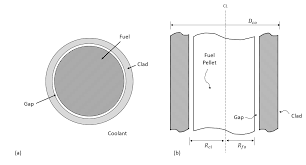
\includegraphics{fuel_pin_schematic.png}
\caption{Schematic of fuel pin geometry.}
\label{fig:fuel_pin_schematic}
\end{marginfigure}

\begin{equation}
\rho c_p \frac{\partial T}{\partial t} = \nabla \cdot k \nabla T + S(\bar{x},t)
\label{eq:heat_eqn}
\end{equation}
where $\rho$ is the material density, $c_p$ is the specific heat, $T$ is temperature, $k$ is the thermal conductivity, and $S(\bar{x},t)$ is a heat source that in general depends on position and time.
\index{thermal diffusivity} \index{heat conduction}
\newthought{The heat equation} is derived based on conservation of energy and represents physical behavior for simple heat conduction problems.  We found solutions assuming uniform and constant thermal diffusivity.\marginnote[-1.75cm]{\textbf{Thermal diffusivity} for a material is defined as $\alpha = \frac{k}{\rho c_p}$.  By assuming constant thermal diffusivity we assumed that $k$, $\rho$ and $c_p$ were constant.}  For the context of conduction in a nuclear fuel pin the temperature profile was found to be:\sidenote{For this solution, in addition to constant thermal diffusivity, the heat source represented by $q^{\prime \prime \prime}$ was assumed to be constant. The equation was cast in polar coordinates with symmetry with respect to angular position and the temperature on the outside surface of the fuel pellet, $T(r_o)$, must be provided as a boundary condition.}
$$T(r) = T(r_o) + \frac{q^{\prime \prime \prime}}{4k}\left(r_o^2 - r^2\right) = T(r_o) + \frac{q^{\prime}}{4 \pi k_{\text{fuel}}}\left(1 - \frac{r^2}{r_o^2} \right) \ \ \ 0 < r < r_o $$
where $r_o$ is the fuel pellet outer radius, $q^{\prime \prime \prime}$ is the heat production rate from fission, and $q^{\prime}$ is the linear heat generation rate.\marginnote[0.5cm]{\textbf{Note: } recall that by definition, $q^{\prime \prime \prime} \pi r^2 L = q^{\prime} L$.} 
This can be re-arranged to solve for the temperature change between the fuel pellet center line and outer surface:
$$T(0) - T(r_o) = \Delta T_{\text{fuel}} = \frac{q^{\prime}}{4 \pi k_{\text{fuel}}}$$

\newthought{Heat conduction from} the fuel to the cladding across the gas-filled gap is modeled as a convective process, where the heat flux $(q^{\prime \prime})$ is proportional to the difference in temperature between the fuel outer radius, $T(r_o)$, and the clad inner radius, $T(r_{ci})$:
$$q^{\prime \prime} = h_{\text{gap}}\left[T(r_o) - T(r_{ci})\right] = h_{\text{gap}} \Delta T_{\text{gap}}$$
where $h_{\text{gap}}$ is called the ``gap conductance'' and represents the convective heat transfer across the pellet-to-clad gap.  Re-arranging the above equation to solve for $\Delta T_{\text{gap}}$ we get:\marginnote{\textbf{Note: } by definition the following relation also holds: $q^{\prime \prime} 2 \pi r L = q^{\prime} L$.}
$$\Delta T_{\text{gap}} = \frac{q^{\prime \prime}}{h_{\text{gap}}} = \frac{q^{\prime}}{2 \pi r_o h_{\text{gap}}}$$
where we take $r_o$ as the reference radius for the heat transfer process.\sidenote{This is a small approximation since, for relevant fuel pins on which this analysis is applied, $r_o$ is very close to $r_{ci}$.}

\newthought{Heat conduction through} the cladding is modeled using, once again, Equation \ref{eq:heat_eqn}.  For the cladding analysis we assumed constant thermal diffusivity and no heat generation in the cladding.\sidenote{This is not quite true: gamma radiation from the fuel deposits a small fraction of its energy in the cladding materials.  We ignored that effect in previous courses and we will ignore it in this course also, I am sad to say. Current computer models used for fuel performance analysis do take non-local gamma energy deposition into account.}
$$T(r) = T(r_{co}) + \frac{q^{\prime}}{2 \pi k_{\text{clad}}}\ln{\left(\frac{r_{co}}{r} \right)}, \ \ \ r_{ci} < r < r_{co}$$
We can, once again, re-arrange this equation to get an expression for $\Delta T_{\text{clad}}$:
$$T(r_{ci}) - T(r_{co}) = \Delta T_{\text{clad}} = \frac{q^{\prime}}{2 \pi k_{\text{clad}}}\ln{\left(\frac{r_{co}}{r_{ci}} \right)}$$

\newthought{Convection to the coolant} on the outer surface of the fuel pin was handled in a similar fashion as convection across the fuel-clad gap:

$$\Delta T_{\text{cool}} = T(r_{co}) - T_{\text{coolant}} = \frac{q^{\prime}}{2 \pi r_{co} h_{\text{cool}}}$$
where $h_{\text{cool}}$ is the convective heat transfer coefficient for the coolant flowing on the outer surface of the rod.  In previous classes, except possibly your heat transfer course, the value of $h_{\text{cool}}$ was taken to be a given parameter.  

\newthought{We can combine} the $\Delta T$'s computed above to get an overall temperature change between the center line of a fuel pellet and the surrounding bulk coolant:

\begin{align*}
\Delta T_{\text{total}} &= \Delta T_{\text{fuel}} + \Delta T_{\text{gap}} + \Delta T_{\text{clad}} + \Delta T_{\text{cool}} \\
&= \frac{q^{\prime}}{2 \pi}\left[\frac{1}{r_{co}h_{\text{cool}}} + \frac{1}{k_{\text{clad}}} \ln{\left(\frac{r_{co}}{r_{ci}} \right)} + \frac{1}{r_o h_{\text{gap}}}+ \frac{1}{2 k_{\text{fuel}}}\right] \\
\end{align*}

\section{Preview for Thermal Section of ER468}
In this course we will elaborate on those previously covered topics.  These ``elaborations'' will capture the following additional physical phenomena:

\begin{itemize}
\item Fuel thermal conductivity is not constant. In fact, fuel thermal conductivity is a function of, among other things:
\begin{enumerate}
\item \textbf{Temperature.}  As $T_{\text{fuel}} \uparrow$, $k(T) \downarrow$. If we re-write the heat equation, making this temperature dependence explicit:
$$ \rho c_{p} \frac{\partial T}{\partial t} = \nabla \cdot k(T) \nabla T + S(\bar{x},t)$$
it becomes apparent that, accounting for this fact, makes the heat equation non-linear.\sidenote{\textbf{Question: } Why does temperature dependent thermal conductivity make the heat equation non-linear?}
\item \textbf{Burn-up.} Burn-up changes the material composition of the fuel through the fission process.  As burn-up proceeds, radiation and long-term exposure to high temperature changes the structural make-up of the fuel. 
\item \textbf{Enrichment.}  This is a small effect, but modern models take it into account.
\item \textbf{Presence of gadolinium.}  Adding gadolinium for reactivity control generally results in somewhat reduced thermal conductivity.  
\item \textbf{Presence of Plutonium.}  Plutonium oxide has many different properties than uranium oxide, including thermal conductivity.\marginnote{\textbf{Note:} For an authoritative description of the chemical, mechanical, and thermal properties of Plutonium, I cannot help but point you to the Plutonium Handbook (7-volume set) available from the American Nuclear Society for \$2400.} 
\end{enumerate}
\item Gap conductance is not constant.  Not to spoil the upcoming lecture, but gap conductance is primarily a function of the gap width.  Gap width changes based on pellet and clad sizing, of course, but also due to pellet dimensional changes during operation and over core life.  As linear power $(q^{\prime})$ increases, the pellet-to-clad gap is reduced and $h_{\text{gap}}$ increases; as the pellet spends time in the core, a variety of changes occur to the oxide structure that result in changes to the gap size.

\item Thermal conductivity of the cladding is not constant.  Like the fuel material, clad material is generally a function of temperature.  Since the clad material does not undergo fission, the thermal conductivity behavior is less complex than for fuel.  Still, since fuel cladding serves as a containment boundary for the fuel material, it is important to accurately model clad behavior and that means temperature-dependent conductivity should be included.

\item Convective heat transfer for fuel assemblies is not a constant.  Modeling convective heat transfer in nuclear reactor fuel assemblies, if all relevant phenomena are taken into account, is very complex.  Fuel assemblies with mixing grids presents some geometric complexity; for light water reactors, the multi-phase flow commonly prevailing in the hottest fuel rod channels is practically impossible to model from first principles.  We will discuss important and relevant correlations available to make use of experimental data that is useful for thermal/hydraulic design.
\end{itemize}
